\documentclass[bibliography=totoc,11pt,BCOR=12mm,DIV=14,twoside,parskip=half,paper=A4,pagesize=auto]{scrbook}\usepackage[]{graphicx}\usepackage{xcolor}
% maxwidth is the original width if it is less than linewidth
% otherwise use linewidth (to make sure the graphics do not exceed the margin)
\makeatletter
\def\maxwidth{ %
  \ifdim\Gin@nat@width>\linewidth
    \linewidth
  \else
    \Gin@nat@width
  \fi
}
\makeatother

\definecolor{fgcolor}{rgb}{0.345, 0.345, 0.345}
\newcommand{\hlnum}[1]{\textcolor[rgb]{0.686,0.059,0.569}{#1}}%
\newcommand{\hlstr}[1]{\textcolor[rgb]{0.192,0.494,0.8}{#1}}%
\newcommand{\hlcom}[1]{\textcolor[rgb]{0.678,0.584,0.686}{\textit{#1}}}%
\newcommand{\hlopt}[1]{\textcolor[rgb]{0,0,0}{#1}}%
\newcommand{\hlstd}[1]{\textcolor[rgb]{0.345,0.345,0.345}{#1}}%
\newcommand{\hlkwa}[1]{\textcolor[rgb]{0.161,0.373,0.58}{\textbf{#1}}}%
\newcommand{\hlkwb}[1]{\textcolor[rgb]{0.69,0.353,0.396}{#1}}%
\newcommand{\hlkwc}[1]{\textcolor[rgb]{0.333,0.667,0.333}{#1}}%
\newcommand{\hlkwd}[1]{\textcolor[rgb]{0.737,0.353,0.396}{\textbf{#1}}}%
\let\hlipl\hlkwb

\usepackage{framed}
\makeatletter
\newenvironment{kframe}{%
 \def\at@end@of@kframe{}%
 \ifinner\ifhmode%
  \def\at@end@of@kframe{\end{minipage}}%
  \begin{minipage}{\columnwidth}%
 \fi\fi%
 \def\FrameCommand##1{\hskip\@totalleftmargin \hskip-\fboxsep
 \colorbox{shadecolor}{##1}\hskip-\fboxsep
     % There is no \\@totalrightmargin, so:
     \hskip-\linewidth \hskip-\@totalleftmargin \hskip\columnwidth}%
 \MakeFramed {\advance\hsize-\width
   \@totalleftmargin\z@ \linewidth\hsize
   \@setminipage}}%
 {\par\unskip\endMakeFramed%
 \at@end@of@kframe}
\makeatother

\definecolor{shadecolor}{rgb}{.97, .97, .97}
\definecolor{messagecolor}{rgb}{0, 0, 0}
\definecolor{warningcolor}{rgb}{1, 0, 1}
\definecolor{errorcolor}{rgb}{1, 0, 0}
\newenvironment{knitrout}{}{} % an empty environment to be redefined in TeX

\usepackage{alltt} % hidelinks
%\let\mathds\mathbb




%\KOMAoptions{BCOR=0mm} % DIV=15,BCOR=12mm

% Farben
%%%%%%%%%%%%%%%%%%%%%%%%%%%%%%%%%

%\usepackage[usenames]{color} %  \textcolor{blue}{blau}
%\usepackage{xcolor}

% Zeichen/Sprache
%%%%%%%%%%%%%%%%%%%%%%%%%%%%%%%%%
\usepackage[german, english]{babel}
\usepackage[utf8]{inputenc}
\usepackage{pdfpages}
\usepackage{lmodern} % avoid warning regarding font sizes, see https://tex.stackexchange.com/questions/58087/how-to-remove-the-warnings-font-shape-ot1-cmss-m-n-in-size-4-not-available
\usepackage{xspace} % needed for shortcut https://tex.stackexchange.com/questions/7793/defining-shortcuts
%\usepackage{autonum} % show numbers for formula only when they are refered to https://tex.stackexchange.com/questions/4728/how-do-i-number-equations-only-if-they-are-referred-to-in-the-text
% Font
% \usepackage[scale=0.9]{tgheros}%% TeX Gyre Sans Serif
% \usepackage{tgtermes}%%           TeX Gyre Times
% \renewcommand{\sfdefault}{qhv} % Bera sans

% Environments
%%%%%%%%%%%%%%%%%%%%%%%%%%%%%%%%%
\usepackage{todonotes}
\usepackage{verbatim} % l?ngere Kommentare mit \begin{comment} ... \end{comment}

% Tabellen
%%%%%%%%%%%%%%%%%%%%%%%%%%%%%%%%%
\usepackage{multicol,multirow}
\usepackage{hhline} % Linien in Tabellen, die kompatibel mit dem Einf?rben der Zellen sind
\usepackage{array}
\newcolumntype{L}[1]{>{\raggedright\let\newline\\\arraybackslash\hspace{0pt}}m{#1}}
\newcolumntype{C}[1]{>{\centering\let\newline\\\arraybackslash\hspace{0pt}}m{#1}}
\newcolumntype{R}[1]{>{\raggedleft\let\newline\\\arraybackslash\hspace{0pt}}m{#1}}
% \usepackage{tabularx}
% \usepackage{booktabs}
% \usepackage{colortbl}                  % F?rben von Zellen in Tabellen
% \usepackage{hhline}

% Graphiken
%%%%%%%%%%%%%%%%%%%%%%%%%%%%%%%%%
%\usepackage{float}
\usepackage[section]{placeins}
% \usepackage{grffile} % ermoglicht punkte/ andere zeichen in dateinamen
% \usepackage{graphicx}
% \usepackage{rotating}
% \usepackage{array}
% %\usepackage{graphpap}
% \usepackage[small, normal]{caption}
% % muss vor subfig stehen, da sonst folgender Fehler auftritt: LaTeX Error: Option clash for package caption
% \usepackage[labelformat=simple, position=top]{subfig}
% \renewcommand{\thesubfigure}{\relax}

% Format
%%%%%%%%%%%%%%%%%%%%%%%%%%%%%%%%%
\usepackage[inner=26mm,outer=21mm,top=28mm,bottom=30mm,includehead]{geometry}
%\usepackage{a4wide} % a4
%\usepackage[inner=26mm,outer=21mm,top=28mm,bottom=36mm,includehead]{geometry}
%\usepackage{setspace}
%\usepackage{lipsum}
%\usepackage{layouts}

% Mathematische Symbole
%%%%%%%%%%%%%%%%%%%%%%%%%%%%%%%%%
\usepackage{amsmath} % mathematische Symbole
\usepackage{amssymb} % \mathfrak{}, \mathbb{R}
\usepackage{amsfonts} % mathematische Symbole => $$ \mathbf{B}, \mathrm{B}, \mathcal{B}, \mathsf{B},
\usepackage{amsthm}
\usepackage{dsfont} % Mathematische Schrifstile - Reele zahlen, complexe Zahlen etc => \mathds{C}
\usepackage{bm} % bold math, allows you to write bold greek letters (both upper and lower case) within
%\usepackage{wasysym} % \ocircle
%\usepackage{eurosym} % => \euro{} zur Darstellung des Euro-Symbols, \EUR{...}
%\usepackage{stmaryrd}
%\usepackage{latexsym}

% Links
%%%%%%%%%%%%%%%%%%%%%%%%%%%%%%%%%
\usepackage{url} % => \url{}
\usepackage[hypertexnames=false, pdfborder={0 0 0}]{hyperref} % Hyperlinks
%\usepackage[hypertexnames=false, bookmarks, linkbordercolor=white, citebordercolor=white, urlbordercolor=white]{hyperref}
% hypertexnames=false bewirkt, dass intern Sections, equations und tables mit 1,2,3,4 ... durchnummeriert werden, verhindert Fehlermeldung: latex destination with the same identifier name equation
% LMU Vorgabe, siehe https://edoc.ub.uni-muenchen.de/help/index.html#property_latex
\hypersetup{
pdfpagemode = {UseNone},
pdftitle = {On Benchmark Experiments and Visualization Methods for the Evaluation and Interpretation of Machine Learning Models},
pdfauthor = {Giuseppe Casalicchio}
}

% Unbekannt
%%%%%%%%%%%%%%%%%%%%%%%%%%%%%%%%%
% \usepackage{ifthen}
% \usepackage{picins}
% \usepackage{bbold}
% \usepackage{fancybox}
\usepackage[inline, shortlabels]{enumitem}
% %\usepackage{float}
% \usepackage{paralist}
% \usepackage{footmisc}
% \renewcommand{\thefootnote}{\fnsymbol{footnote}}

% Literatur
%%%%%%%%%%%%%%%%%%%%%%%%%%%%%%%%%
%\usepackage{pifont} %  Pfeil bei Referenzen
\usepackage[round]{natbib} % => \bibliographystyle{ } und \bibliography{ }
\bibliographystyle{chicago} % apalike
%\usepackage{bibentry}
%\usepackage{chapterbib} % to include multiple bib files
%\usepackage[resetlabels,labeled]{multibib}
%\newcites{New}{The other list}

% Table of Contents
%%%%%%%%%%%%%%%%%%%%%%%%%%%%%%%%%
% Avoid bad box in TOC due to page number with three digits (i.e., page numbers > 99)
% https://tex.stackexchange.com/questions/49887/overfull-hbox-warning-for-toc-entries-when-using-memoir-documentclass
\makeatletter
\renewcommand{\@pnumwidth}{2em}
\renewcommand{\@tocrmarg}{3em}
\makeatother

%\usepackage{titletoc}
%\titlecontents{part}[0pt]{\vspace{15pt}\large\bfseries}{\contentslabel{1.8em}}{\hspace*{0em}}{\hfill\contentspage}[\smallskip]
%\titlecontents{section}[3.6em]{}{\contentslabel{1.8em}}{\hspace*{0em}}{\titlerule*[1pc]{.}\contentspage}
%\titlecontents{subsection}[4.65em]{}{\contentslabel{2.85em}}{\hspace*{0em}}{\titlerule*[1pc]{.}\contentspage}
%\titlecontents{subsubsection}[8.35em]{}{\contentslabel{3.75em}}{\hspace*{0em}}{\titlerule*[1pc]{.}\contentspage}

%\usepackage{chngcntr}
%\counterwithin*{chapter}{part}
% \titlecontents{part}[0pt]{\normalsize\bfseries\protect\addvspace{15pt}}%
% {\contentslabel{1.8em}}{\partname{ }}%
% {\hfill \contentspage}%

% \makeatletter
% \renewcommand*{\l@part}[2]{%
% \par\addvspace{\topsep}
% \setlength\@tempdima{2.3em}%
% \noindent\hspace*{1.5em}\textbf{#1}\par}
% \makeatother

% Header Definition
%%%%%%%%%%%%%%%%%%%%%%%%%%%%%%%%%
% header giuseppe
% \usepackage[automark,headsepline]{scrlayer-scrpage}
% \pagestyle{scrheadings}
% \lehead[]{\pagemark}
% \rehead[]{\leftmark}
% \lohead[]{\leftmark}
% \rohead[]{\pagemark}
% \lefoot[]{}\refoot[]{}\lofoot[]{}\rofoot[]{}
\usepackage{silence} % Verhindert warning fancyhdr + KOMA Klasse
\WarningFilter{scrbook}{Usage of package `fancyhdr'}

% add pagenumber to chapter pages
% \WarningFilter{scrbook}{Usage of package `titlesec'}
% \usepackage{titlesec}
% \assignpagestyle{\chapter}{fancyplain}

\usepackage{fancyhdr}
\pagestyle{fancyplain}
\renewcommand{\chaptermark}[1]
{\markboth{\thechapter.\ #1}{}}
\renewcommand{\sectionmark}[1]
{\markright{\thesection\ #1}}

% header felix
%\lhead[\fancyplain{}{\bfseries\thepage}]{\fancyplain{}{\bfseries\rightmark}}
%\rhead[\fancyplain{}{\bfseries\leftmark}]{\fancyplain{}{\bfseries\thepage}}

% header stephi
\newcommand{\helv}{
\fontfamily{phv}\fontseries{b}\fontsize{10}{10}\selectfont
}
%{\fontsize{Fontgr??e}{Grundlinienabstand}\selectfont}
\lhead[\fancyplain{}{}]{\fancyplain{}{\helv\rightmark}}
\rhead[\fancyplain{}{\helv\leftmark}]{\fancyplain{}{}}
%\lhead[\fancyplain{}{\helv\thepage}]{\fancyplain{}{\helv\rightmark}}
%\rhead[\fancyplain{}{\helv\leftmark}]{\fancyplain{}{\helv\thepage}}
%\lhead[\fancyplain{}{\helv\rightmark}]{\fancyplain{}{\helv\thepage}}
%\rhead[\fancyplain{}{\helv\thepage}]{\fancyplain{}{\helv\leftmark}}
\renewcommand*{\partpagestyle}{empty}
\lfoot[\helv\thepage]{}
\rfoot[]{\helv\thepage}
\cfoot{}

% Optionen / Settings
%%%%%%%%%%%%%%%%%%%%%%%%%%%%%%%%%
\setlength{\topmargin}{0mm}
\sloppy

% Hurenkinder und Schusterjungen verhindern
\clubpenalty = 10000
\widowpenalty = 10000
\displaywidowpenalty = 10000

% Verhindere warning wegen Einbinden neuerer PDF versionen (siehe https://tex.stackexchange.com/questions/270218/includegraphicspdf-image-is-dropping-items-comments-from-the-pdf-image)
%\pdfminorversion = 7

% LatexMath definitions
\usepackage{xargs}

%\DeclareMathOperator*{\argmin}{arg\,min}
%\newcommand{\argmin}{\operatornamewithlimits{arg\,min}}
\newcommand{\argmin}{\mathop{\mathrm{arg\,min}}}

% basic probability + stats
\renewcommand{\P}{\mathds{P}}                                               % P, probability
\newcommand{\E}{\mathds{E}}                                                 % E, expectation
\newcommand{\var}{\mathsf{Var}}                                             % Var, variance
\newcommand{\cov}{\mathsf{Cov}}                                             % Cov, covariance
\newcommand{\corr}{\mathsf{Corr}}                                           % Corr, correlation
\newcommand{\normal}{\mathcal{N}}                                           % N of the normal distribution
\newcommand{\iid}{\overset{i.i.d}{\sim}}                                    % dist with i.i.d superscript
\newcommand{\distas}[1]{\overset{#1}{\sim}}                                 % ... is distributed as ...

% sets
\renewcommand{\S}{S}
\newcommand{\Spi}[1][j]{B_{#1} (\pi)}
\newcommand{\Scpi}[1][j]{A_{#1} (\pi)}
\newcommand{\Sc}{C}
\newcommand{\Sj}{\S \cup \{j\}}
\newcommand{\pairs}[1]{\{ (#1) \}}

\newcommand{\Lswitch}[1][\Xperm_{\S}]{L (\fh (#1, \XC ), Y)}
\newcommand{\Eswitch}{\E (\Lswitch)} %\E_{\Xperm_\S}(GE(\fh(\Xperm_\S, X_{\Sc})))
\newcommand{\Eorig}{\E (L (\fh (X), Y)) } %GE(\fh(X_\S, X_{\Sc}))
											% xi, slack variable (SVM)

% machine learning

%%%%%% ml - data
\newcommand{\Xspace}{\mathcal{X}}                                           % X, input space
\newcommand{\Yspace}{\mathcal{Y}}                                           % Y, output space
\newcommand{\X}{\mathbf{X}}
\newcommand{\nset}{\{1, \ldots, n\}}                                        % set from 1 to n
\newcommand{\pset}{\{1, \ldots, p\}}                                        % set from 1 to p
\newcommand{\gset}{\{1, \ldots, g\}}                                        % set from 1 to g
\newcommand{\Pxy}{\P_{xy}}                                                  % P_xy
% observation (x, y)
\newcommand{\xvec}{(x_1, \ldots, x_p)^\top}                                 % (x1, ..., xp)
\newcommand{\xivec}{(x^{(i)}_1, \ldots, x^{(i)}_p)^\top}                    % (x1^i, ..., xp^i)
\renewcommand{\xi}[1][(i)]{\mathbf{x}^{#1}}                                          % x^i
\newcommand{\xis}[1][(i)]{\mathbf{x}_{\S}^{#1}}                                          % x^i
\newcommand{\zi}[1][(i)]{\mathbf{z}^{#1}}
\newcommand{\zis}[1][(i)]{\mathbf{z}_{\S}^{#1}}                                          % x^i
\newcommand{\zic}[1][(i)]{\mathbf{z}_{\Sc}^{#1}}                                          % x^i
\newcommand{\xic}[1][(i)]{\mathbf{x}_{\Sc}^{#1}}                                          % x^i
\newcommand{\xij}{x_j^{(i)}}
\newcommand{\yi}[1][(i)]{y^{#1}}                                            % y^i
\newcommand{\xyi}{(\xi, \yi)}                                               % (x^i, y^i)
\newcommand{\xy}{(x, y)}                                                    % (x, y)
% data
\newcommand{\D}{\mathcal{D}}                                                % D, data
%\newcommand{\Dset}{\{ (\mathbf{x}^{(1)}, y^{(1)}), \ldots, (\mathbf{x}^{(n)},  y^{(n)})\}}    % {(x1,y1)), ..., (xn,yn)} data
\newcommand{\Dset}[1][n]{\pairs{ \mathbf{x}^{(i)}, y^{(i)} }_{i=1}^{#1}}    % {(x1,y1)), ..., (xn,yn)} data
\newcommand{\xdat}{\{ x^{(1)}, \ldots, x^{(n)}\}}   						            % {x1, ..., xn} data
\newcommand{\Dtrain}{\mathcal{D}_{\text{train}}}                            % D_train, training set
\newcommand{\Dtest}{\mathcal{D}_{\text{test}}}                              % D_test, test set
\newcommand{\xj}{\mathbf{x}_j}                                              % x_j (bold)
\newcommand{\xone}{\mathbf{x}_1}                                              % x_j (bold)
\newcommand{\xp}{\mathbf{x}_p}                                              % x_j (bold)
\newcommand{\xS}{\mathbf{x}_S}                                              % x_S (bold)
\newcommand{\xC}{\mathbf{x}_{\Sc}}                                              % x_S (bold)
\newcommand{\Xperm}{\tilde{X}}
\newcommand{\XC}{X_{\Sc}}
\newcommand{\XS}{X_{\S}}
\newcommand{\xjvec}{(x^{(1)}_j, \ldots, x^{(n)}_j)^\top}                    % (x^1_j, ..., x^p_j)
\newcommand{\ydat}{\mathbf{y}}                                              % y (bold)
\newcommand{\yvec}{(y^{(1)}, \hdots, y^{(n)})^\top}                         % (y1, ..., yn)

%%%%%% ml - model
% prediction function f, theta, yhat
\newcommand{\Hspace}{H}
\newcommand{\fx}{f(x)}                                                      % f(x)
\newcommand{\fxh}{\fh(\mathbf x)}                                                   % fhat(x)
\newcommand{\fxt}{f(x | \theta)}                                            % f(x | theta)
\newcommand{\fxi}{f(\xi)}                                                   % f(x^(i))
\newcommand{\fxih}{\hat{f}(\xi)}                                              % f(x^(i))
\newcommand{\fxit}{f(x^{(i)} | \theta)}                                     % f(x^(i) | theta)
\newcommand{\fh}{\hat{f}}                                                   % f hat
\newcommand{\fhS}{\fh_{\S}}
\newcommand{\fS}{f_{\S}}
\newcommand{\fhSi}{\fhS^{(i)}}
\newcommand{\thetah}{\hat{\theta}}                                          % theta hat
\newcommand{\fhD}{\fh_{\D}}                                                 %
\newcommand{\fhDtrain}{\fh_{\Dtrain}}                                       %

\newcommand{\MR}{PFI}
\newcommand{\hMR}{\widehat{\MR}}
\newcommand{\MRS}[1][\S]{\MR_{#1}}
\newcommand{\hMRS}[1][\S]{\hMR_{#1}}
\newcommand{\hMRSa}[1][\S]{\hMR_{#1, \text{approx}}}
%\newcommand{\w}[1][\S]{v_{#1}(\fh, \Dtest)}
\newcommand{\w}[1][(\S)]{v_{GE}#1}
%\newcommand{\Lii}{\Li[(i)]} % L(\fh(\xi), \yi)
%\newcommandx{\Li}[2][1=(k), 2=(i)]{L^{#2}(\fh, \xis[#1])}

\newcommand{\Lii}{L(\fh(\xi), \yi)}
\newcommandx{\Li}[3][1=(k), 2=(i), 3=(i)]{L(\fh(\xis[#1], \xic[#2]), y^{#3})}

\newcommand{\mfeat}{m_{\textnormal{feat}}}
\newcommand{\mobs}{m_{\textnormal{obs}}}

\newcommand{\hPI}{\widehat{PI}_{\S}} %  \widehat{\MR}_{\S}
\newcommand{\PI}[1][\S]{PI_{#1}}
\newcommand{\ICI}{\hMRS^{(i)}}
\newcommand{\ICIvar}[1][(i)]{\MRS^{#1}}
%\newcommandx{\PFIikS}[3][1=\xi, 2=\mathbf{x}_{\S}^{(k)}, 3=\S]{PFI_{#3} (#1, #2)}
%\newcommand{\PFIikS}[1][(k)]{\widehat{\MR}^{(i)} (\xis[#1])} % was used until 29.3
\newcommandx{\PFIikS}[2][1=(i), 2=(k)]{\Delta L^{#1} (\xis[#2])}
%\newcommand{\PFIikS}{\widehat{\MR}^{(i)} (\xis[(k)])}
\newcommand{\yh}{\hat{y}}                                                   % y hat for prediction of target
\newcommand{\yih}{\hat{y}}                                                  % y hat for prediction of target
% prediction function h
\newcommand{\hx}{h(x)}                                                      % h(x)
\newcommand{\hxt}{h(x | \theta)}                                            % h(x | theta)
\newcommand{\hxi}{h(\xi)}                                                   % h(x^(i))
\newcommand{\hxit}{h(x^{(i)} | \theta)}                                     % h(x^(i) | theta)
\newcommand{\hh}{\hat{h}}                                                   % h hat
\newcommand{\hxh}{\hat{h}(x)}                                               % hhat(x)
% risk
% pdf of x and (x,y)
\newcommand{\post}{\P(y = 1 | x)}                                           % P(y = 1 | x), post. prob for y=1
\newcommand{\postk}{\P(y = k | x)}                                          % P(y = k | y), post. prob for y=k
\newcommand{\pik}{\pi_k}                                                    % pi_k, prior
\newcommand{\pix}{\pi(x)}                                                   % pi(x), P(y = 1 | x)
\newcommand{\pixt}{\pi(x | \theta)}                                          %
\newcommand{\pikx}{\pi_k(x)}                                                % pi_k(x), P(y = k | x)
\newcommand{\pikxt}{\pi_k(x | \theta)}                                       %
\newcommand{\pijx}{\pi_j(x)}                                                % pi_j(x), P(y = j | x)
\newcommand{\pixh}{\hat \pi(x)}                                             % pi(x) hat, P(y = 1 | x) hat
\newcommand{\pikxh}{\hat \pi_k(x)}                                          % pi_k(x) hat, P(y = k | x) hat
\newcommand{\pdf}{p}                                                        % p
\newcommand{\pdfx}{p(x)}                                                    % p(x)
\newcommand{\pdfxy}{p(x,y)}                                                 % p(x, y)
\newcommand{\pdfxyt}{p(x, y | \theta)}                                      % p(x, y | theta)
\newcommand{\pdfxyit}{p(\xi, \yi | \theta)}                                 % p(x^(i), y^(i) | theta)
\newcommand{\pdfxyk}{p(x | y=k)}                                            % p(x | y = k)
\newcommand{\pdfxiyk}{p(\xi | y=k)}                                         % p(x^i | y = k)
\newcommand{\lpdfxyk}{\log \pdfxyk}                                         %
\newcommand{\lpik}{\log \pik}                                               %
\newcommand{\pdfygxt}{p(y |x, \theta)}                                      % p(y | x, theta)
\newcommand{\pdfyigxit}{p(\yi |\xi, \theta)}                                % p(y^i |x^i, theta)
\newcommand{\lpdfygxt}{\log \pdfygxt }                                      %
\newcommand{\lpdfyigxit}{\log \pdfyigxit}                                   %

% residual and margin
\newcommand{\eps}{\epsilon}                                                 % residual, stochastic
\newcommand{\epsi}{\epsilon^{(i)}}                                          % r^i, residual, stochastic
\newcommand{\epsh}{\hat{\epsilon}}                                          % residual, estimated
\newcommand{\epshi}{\hat{\epsilon}^{(i)}}
\newcommand{\yf}{y \fx}                                                     % y f(x), margin
\newcommand{\yfi}{\yi \fxi}                                                 % y^i f(x^i), margin
\newcommand{\Sigmah}{\hat \Sigma}									                      		% estimated covariance matrix
\newcommand{\Sigmahj}{\hat \Sigma_j}									                    	% estimated covariance matrix for the j-th class

% ml - loss, risk, likelihood
\newcommand{\Lxy}{L(y, f(x))}                                               % L(y, f(x))
\newcommand{\Lxyi}{L(\yi, \fxi)}                                            % L(y^i, f(x^i))
\newcommand{\Lxyt}{L(y, \fxt)}                                              % L(y, f(x | theta))
\newcommand{\Lxyit}{L(\yi, \fxit)}                                          % L(y^i, f(x^i | theta)
\newcommand{\risk}{\mathcal{R}}                                             % R
\newcommand{\riskf}{\risk(f)}                                               % R(f)
\newcommand{\riske}{\mathcal{R}_{\text{emp}}}                               % R_emp
\newcommand{\riskef}{\riske(f)}                                             % R_emp(f)
\newcommand{\risket}{\mathcal{R}_{\text{emp}}(\theta)}                      % R_emp(theta)
\newcommand{\riskr}{\mathcal{R}_{\text{reg}}}                               % R_reg
\newcommand{\riskrt}{\mathcal{R}_{\text{reg}}(\theta)}                      % R_reg(theta)
\newcommand{\riskrf}{\riskr(f)}                                             % R_reg(f)
\newcommand{\LL}{\mathcal{L}}                                               % L, likelihood
\newcommand{\LLt}{\mathcal{L}(\theta)}                                      % L(theta), likelihood
\renewcommand{\ll}{\ell}                                                    % l, log-likelihood
\newcommand{\llt}{\ell(\theta)}                                             % l(theta), log-likelihood
\newcommand{\LS}{\mathfrak{L}}                                              % ????????????
\newcommand{\TS}{\mathfrak{T}}                                              % ??????????????
\newcommand{\errtrain}{\text{err}_{\text{train}}}                           % training error
\newcommand{\errtest}{\text{err}_{\text{test}}}                             % training error
\newcommand{\errexp}{\overline{\text{err}_{\text{test}}}}                   % training error

% resampling
\newcommand{\GE}[1]{GE(\fh_{#1})}                                           % Generalization error GE
\newcommand{\GEh}[1]{\widehat{GE}_{#1}}                                     % Estimated train error
\newcommand{\GED}{\GE{\D}}                                                  % Generalization error GE
\newcommand{\EGEn}{EGE_n}                                                  % Generalization error GE
\newcommand{\EDn}{\E_{|\D| = n}}                                                  % Generalization error GE


%%%%%%%%%%%%%%%%%%%%%%%%%%%%%%%%%
%  Deckblatt + Titelseite

% The content to be shown in the PDF can be specified below after begin{document}
\newcommand{\Title}[9]{
  % outer title
  \frontmatter %\AddToShipoutPicture*{\Front}
  \thispagestyle{empty}
  \begin{flushleft}

    \sffamily
    \Large #2 \\
    \vspace{2.1cm}
    \huge \textbf{#1}\\ \vspace{.8cm}
    \normalsize Dissertation an der Fakult\"at f\"ur #3 \\
    der Ludwig-Maximilians-Universit\"at M\"unchen \\ \vspace{.3cm}
    Eingereicht am #4

  \end{flushleft}
  \cleardoublepage

  \pagenumbering{roman}
  % inner title
  \thispagestyle{empty}
  \begin{flushleft}

    \sffamily
    \Large #2 \\ \vspace{2.1cm}
    \huge \textbf{#1}\\ \vfill
    \large Dissertation an der Fakult\"at f\"ur #3 \\
    der Ludwig-Maximilians-Universit\"at M\"unchen
    \\ [11.5mm]
    Eingereicht am #4

  \end{flushleft}

  \newpage
  \thispagestyle{empty}
  \begin{flushleft}

    \vspace*{\stretch{1}}
    \sffamily \large
    Erster Berichterstatter:  #5 \\
    Zweiter Berichterstatter: #6 \\
    Dritter Berichterstatter:  #7 \\ [11.5mm]
    Tag der Disputation: #8

  \end{flushleft}
  \newpage
}
\newcommand{\deadline}{07.01.2019}

%%%%%%%%%%%%%%%%%%%%%%%%%%%%%%%%%
% Contributions

% shortcut that can be used to refer to your publications
\newcommand{\contb}{Chapter \ref{chap:cont2}\xspace}%: Multilabel Classification with \textsf{R} Package \textsf{mlr}}
\newcommand{\contc}{Chapter \ref{chap:cont3}\xspace}%: \textsf{OpenML}: An \textsf{R} package to connect to the machine learning platform}
\newcommand{\contd}{Chapter \ref{chap:cont4}\xspace}%: OpenML Benchmarking Suites and the OpenML100}
\newcommand{\conte}{Chapter \ref{chap:cont5}\xspace}%: The Residual-Based Predictiveness Curve}
\newcommand{\contf}{Chapter \ref{chap:cont6}\xspace}%: Visualizing the Feature Importance for Black Box Models}

% shortcut that is shown before the publication is embedded in the '03-attached-contributions-parts.Rnw'
\newcommand{\citationb}{
Probst, P., Au, Q., Casalicchio, G., Stachl, C., and Bischl, B. (2017).
\newblock {Multilabel Classification with R Package mlr}.
\newblock {\em R Journal}, 9(1).
\newblock {\em \url{https://journal.r-project.org/archive/2017/RJ-2017-012/index.html}\/}.
}
\newcommand{\citationc}{
Casalicchio, G., Bossek, J., Lang, M., Kirchhoff, D., Kerschke, P., Hofner, B.,
  Seibold, H., Vanschoren, J., and Bischl, B. (2017).
\newblock {OpenML: An R Package to Connect to the Machine Learning Platform OpenML}.
\newblock {\em Computational Statistics}, pages 1--15.
\newblock {\em \url{https://doi.org/10.1007/s00180-017-0742-2}\/}.
}
\newcommand{\citationd}{
Bischl, B., Casalicchio, G., Feurer, M., Hutter, F., Lang, M., Mantovani,
  R.~G., van Rijn, J.~N., and Vanschoren, J. (2017).
\newblock {OpenML Benchmarking Suites and the OpenML100}.
\newblock {\em arXiv preprint arXiv:1708.03731}.
\newblock {\em \url{https://arxiv.org/abs/1708.03731}\/}.
\newblock In Preparation.
}
\newcommand{\citatione}{
Casalicchio, G., Bischl, B., Boulesteix, A.-L., and Schmid, M. (2016).
\newblock {The Residual-based Predictiveness Curve: A Visual Tool to Assess the
  Performance of Prediction Models}.
\newblock {\em Biometrics}, 72(2):392--401.
\newblock {\em \url{https://doi.org/10.1111/biom.12455}\/}.
}
\newcommand{\citationf}{
Casalicchio, G., Molnar, C., and Bischl, B. (2018).
\newblock {Visualizing the Feature Importance for Black Box Models}.
\newblock {\em arXiv preprint arXiv:1804.06620}.
\newblock {\em \url{https://arxiv.org/abs/1804.06620}\/}.
\newblock To Appear in: {\em Machine Learning and Knowledge Discovery in Databases: European Conference, ECML PKDD 2018}.
}
\IfFileExists{upquote.sty}{\usepackage{upquote}}{}
\begin{document}
%%%%%%%%%%%%%%%%%%%%%%%%%%%%%%%%%
% Frontmatter
\Title
{On Benchmark Experiments and Visualization Methods for the Evaluation and Interpretation of Machine Learning Models}% 1  title
{Giuseppe Casalicchio}                    % 2  your name
{Mathematik, Informatik und Statistik}    % 3  faculty
{\deadline}                               % 4  date of submission
{Prof. Dr. Bernd Bischl}                  % 5  1st referee
{Prof. Dr. Friedrich Leisch}              % 6  2nd referee
{PD Dr. Fabian Scheipl}                   % 7  3nd referee
{18.03.2019}                              % 8  date of defense (not relevant/known yet)

%\pagenumbering{Roman}

%%%%%%%%%%%%%%%%%%%%%%%%%%%%%%%%%
% Acknowledgments



\thispagestyle{empty}
\section*{Acknowledgments}
\textit{This thesis would not have been possible without the help, support, guidance, and advice of many people!
In particular, I would like to express my sincere gratitude to} $\dots$

\begin{itemize}
\item[$\dots$] \textit{my supervisor Prof. Dr. Bernd Bischl for the seamless collaboration, trust, support, encouragement and many advice throughout the years.}
\item[$\dots$] \textit{Prof. Dr. Friedrich Leisch and PD Dr. Fabian Scheipl for their willingness to act as the second and third reviewer for my Ph.D. thesis.}
\item[$\dots$] \textit{Prof. Dr. Christian Heumann and Prof. Dr. Helmut Küchenhoff for their availability to be part of the examination panel at my Ph.D. defense.}
\item[$\dots$] \textit{Prof. Dr. Matthias Schmidt for the excellent supervision and guidance in my first research project.}
\item[$\dots$] \textit{Prof. Dr. Helmut Küchenhoff for the financial support during my work at the StabLab, which gave me the opportunity to work on many interesting consulting projects.}
\item[$\dots$] \textit{the Centre Digitisation.Bavaria (ZD.B) and the LMUexcellent program for financial support during my work on these projects.}
\item[$\dots$] \textit{Prof. Dr. Joaquin Vanschoren and Jan van Rijn for pushing forward the OpenML project and organizing many delightful workshops and hackathons with lots of free lunches.}
\item[$\dots$] \textit{all my coauthors for the fruitful collaborations.}
\item[$\dots$] \textit{all members of my working group: Thank you for the great collaboration, inspiring discussions and unforgettable time at different workshops and conferences!}
\item[$\dots$] \textit{all current and former office colleagues: Thank you Lisa Möst, Janek Thomas, Xudong Sun, Daniel Schalk, Stefan Coors for withstanding all my noises and monologues in the office.}
\item[$\dots$] \textit{all remaining former and current colleagues at the Department of Statistics for the excellent general atmosphere.}
\item[$\dots$] \textit{my parents and the best girlfriend who always support me, understand me (most of the time) and are always there for me.}
\end{itemize}
\newpage

\cleardoublepage

%%%%%%%%%%%%%%%%%%%%%%%%%%%%%%%%%
% Summary



\thispagestyle{empty}
\section*{Zusammenfassung}

Zusammenfassung

\cleardoublepage




\thispagestyle{empty}
\section*{Summary}

Summary

\cleardoublepage

%%%%%%%%%%%%%%%%%%%%%%%%%%%%%%%%%
% Contents
%\pagenumbering{roman}
%\pagestyle{empty}
%\pagenumbering{gobble}
{\small \tableofcontents}
\cleardoublepage

%%%%%%%%%%%%%%%%%%%%%%%%%%%%%%%%%
% Body
\pagenumbering{arabic}
\mainmatter\setcounter{page}{1}
%\part{Introduction and Background}



\chapter{Introduction}

\section{Outline}
% What is the thesis about
This thesis focuses on topics no one will ever read.

% Explain chapter 1 (Outline & Motivation)
The next section gives an overview of all contributing articles and describes their respective goals on a general level.
Furthermore, the section presents the motivation of the contributing articles, and it establishes a connection between the articles from a general perspective.

% Explain chapter 2
Chapter \ref{chap:background} introduces some basic concepts that help with understanding the broader context of this thesis, and it outlines previous and related work.
The contents of the chapter should be understood as a guideline for the reader regarding the main topics of this thesis.
In particular, this chapter also points out how the individual contributions of this thesis fit within the context of the topics.
It should be noted that the notation used in Chapter \ref{chap:background} has been unified and therefore does not always match the notation used in the contributing articles embedded in Chapters \ref{chap:cont2} to \ref{chap:cont6}.
However, the analogies in the notation should be clear from the context.

% Explain part I - IV
The rest of this thesis is organized into three main parts (i.e., Part \ref{part:mlr} - \ref{part:iml}).
The contributing articles of this thesis are embedded within these parts as chapters (i.e., Chapter \ref{chap:cont2} - \ref{chap:cont6}).
At the beginning of each of these chapters, the full reference to the original publication is given, including a description of the author's specific contributions.
If applicable, other information such as supplementary materials, accompanying software, and copyright information of the articles are also included.
The thesis concludes with Part \ref{part:conclusion} by emphasizing possible future and ongoing work.

\section{Motivation and Scope}

Motivate your thesis and describe its scope




\chapter{Methodological and General Background}
\label{chap:background}




\section{Performance Measures}
\label{sec:perfmeasures}

Blabla

\subsection{Measures for Regression}

Blabla

\subsection{Measures for Binary Classification}
\label{sec:binclass}

Blabla with nice picture

\begin{figure}[!htb]
\centering
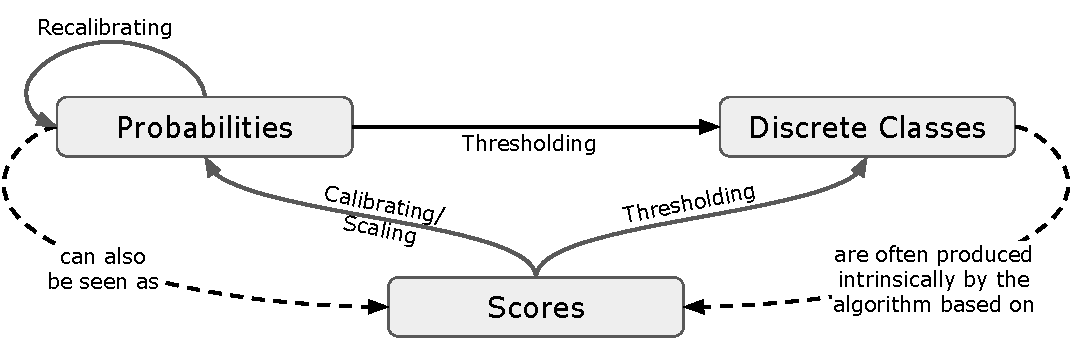
\includegraphics[width=0.7\textwidth]{figures/classifier-predictions_large.pdf}
\caption{Illustration of how different types of predictions can be converted into another type. The topics of recalibrating, calibrating, and thresholding are also referred to in the corresponding paragraphs below.}\label{fig:classifpred}
\end{figure}

\subsubsection*{Discrete Classifiers}

Blabla with nice table

\begin{table}[!htb]
\begin{center}
\renewcommand{\arraystretch}{1.2}
\begin{tabular}{l|c|c|c|c}
\multicolumn{2}{c}{} & \multicolumn{2}{c}{Ground Truth} & \\
\cline{3-4}
\multicolumn{2}{c|}{} & Positive & Negative & \\
\multicolumn{2}{c|}{} & $Y = 1$ & $Y = 0$ & \\
\cline{2-4}
\parbox[t]{4mm}{\multirow{4}{*}{\rotatebox[origin=c]{90}{Prediction}}}
%& & & & \\
& Positive & \multirow{2}{*}{$TP$} & \multirow{2}{*}{$FP$} & \\
& $\hh(X) = 1$ & & & \\
\cline{2-4}
%& & & & \\
& Negative & \multirow{2}{*}{$FN$} & \multirow{2}{*}{$TN$} & \\
& $\hh(X) = 0$ & & & \\
\cline{2-4}
\multicolumn{1}{c}{} & \multicolumn{1}{c|}{Total} & \multicolumn{1}{c|}{$TP + FN$} & \multicolumn{1}{c|}{$FP + TN$} & \\
\end{tabular}
\end{center}
\caption{An illustration of a $2 \times 2$ confusion matrix.
$TN$ and $TP$ refer to the number of predicted classes that were correctly classified as the negative and positive class, respectively.
$FN$ and $FP$ refer to the positive and negative classes of the ground truth that were wrongly classified as the negative and positive class, respectively.}\label{tab:confusion}
\end{table}

% Add more sections here if needed

\part{Machine Learning Software in \textsf{R}}
\label{part:mlr}

\chapter{Multilabel Classification with \textsf{R} Package \textsf{mlr}}
\label{chap:cont2}

Chapter \ref{chap:cont2} describes several methods for multilabel classification that were also implemented into our \textsf{R} package \textsf{mlr} \citep{Bischl2016}.
Furthermore, the methods are compared in a benchmark study on several multilabel datasets using different observation-based multilabel performance measures.

\subsubsection*{Contributing article:}

\citationb

\subsubsection*{Copyright information:}

This article is licensed under a \href{https://creativecommons.org/licenses/by/4.0}{Creative Commons Attribution 4.0 International license} (\url{https://creativecommons.org/licenses/by/4.0/}).

\subsubsection*{Author contributions:}

Explain what you and others did.

\subsubsection*{Supplementary material available at:}

\begin{itemize}
\item Supplementary material: \url{https://doi.org/10.6084/m9.figshare.3384802.v5}
\item Tutorial: \url{https://mlr.mlr-org.com/articles/tutorial/multilabel.html}
\item The \textsf{mlr} package:
\begin{itemize}
\item Paper: \url{http://jmlr.org/papers/v17/15-066.html}
\item \textsf{R} package: \url{https://github.com/mlr-org/mlr}
\end{itemize}
\end{itemize}




\newpage
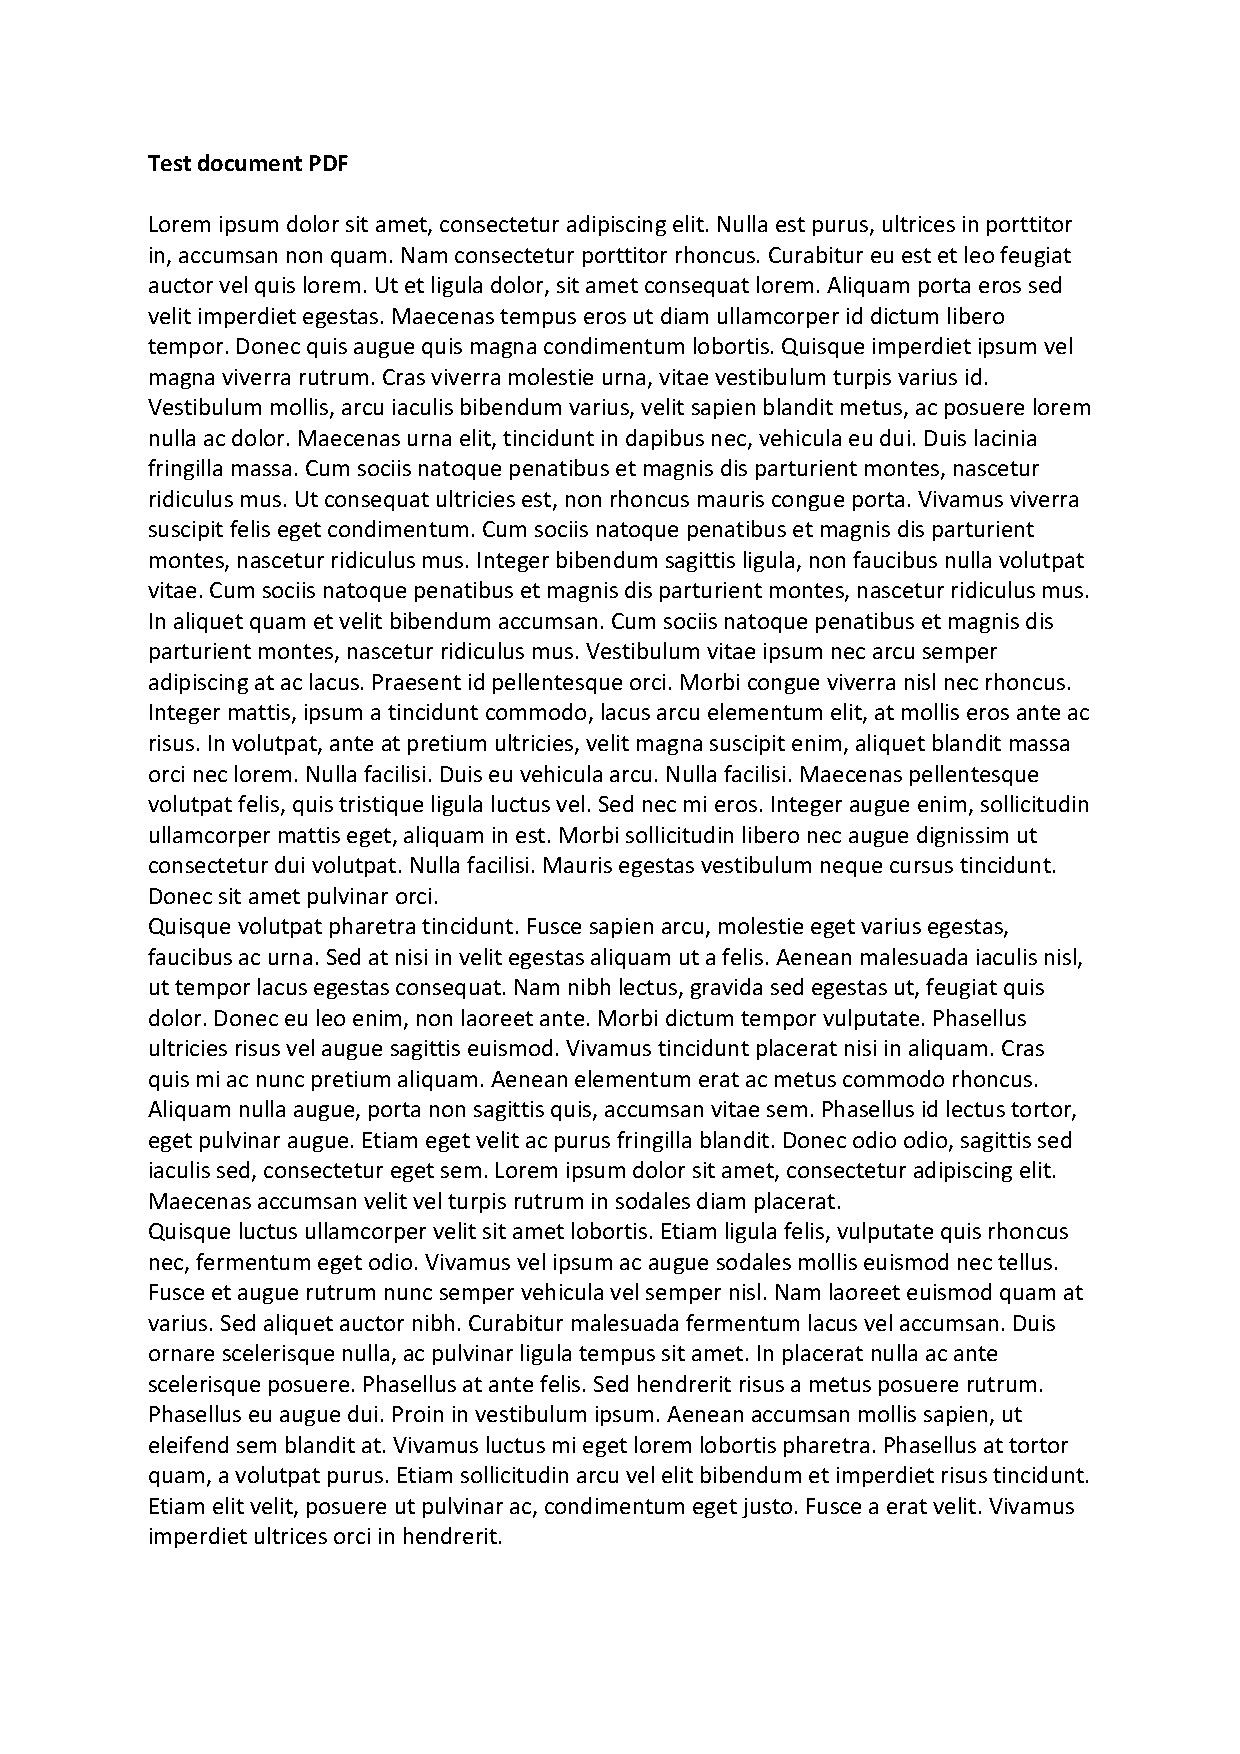
\includepdf[pages={1-last}, pagecommand={\pagestyle{fancyplain}}, width=0.98\textwidth, clip, trim=14mm 8mm 14mm 8mm, offset=0 -6mm]{contribution2-multilabel.pdf}



\part{On Benchmark Experiments with OpenML}
\label{part:bench}

\chapter{\textsf{OpenML}: An \textsf{R} Package to Connect to the Machine Learning Platform OpenML}
\label{chap:cont3}

Chapter \ref{chap:cont3} introduces the \textsf{R} package \textsf{OpenML}, which provides a simple interface for communicating with the OpenML server directly from within \textsf{R} and allows users to easily search, download, and upload datasets and benchmark results.

\subsubsection*{Contributing article:}

\citationc

\subsubsection*{Copyright information:}

Springer-Verlag GmbH Germany, 2017.

\subsubsection*{Author contributions:}

Explain what you and others did.

\subsubsection*{Supplementary material available at:}

\begin{itemize}
\item \textsf{R} package: \url{https://github.com/openml/openml-r}
\item Tutorial: \url{http://openml.github.io/openml-r}
\end{itemize}



\newpage
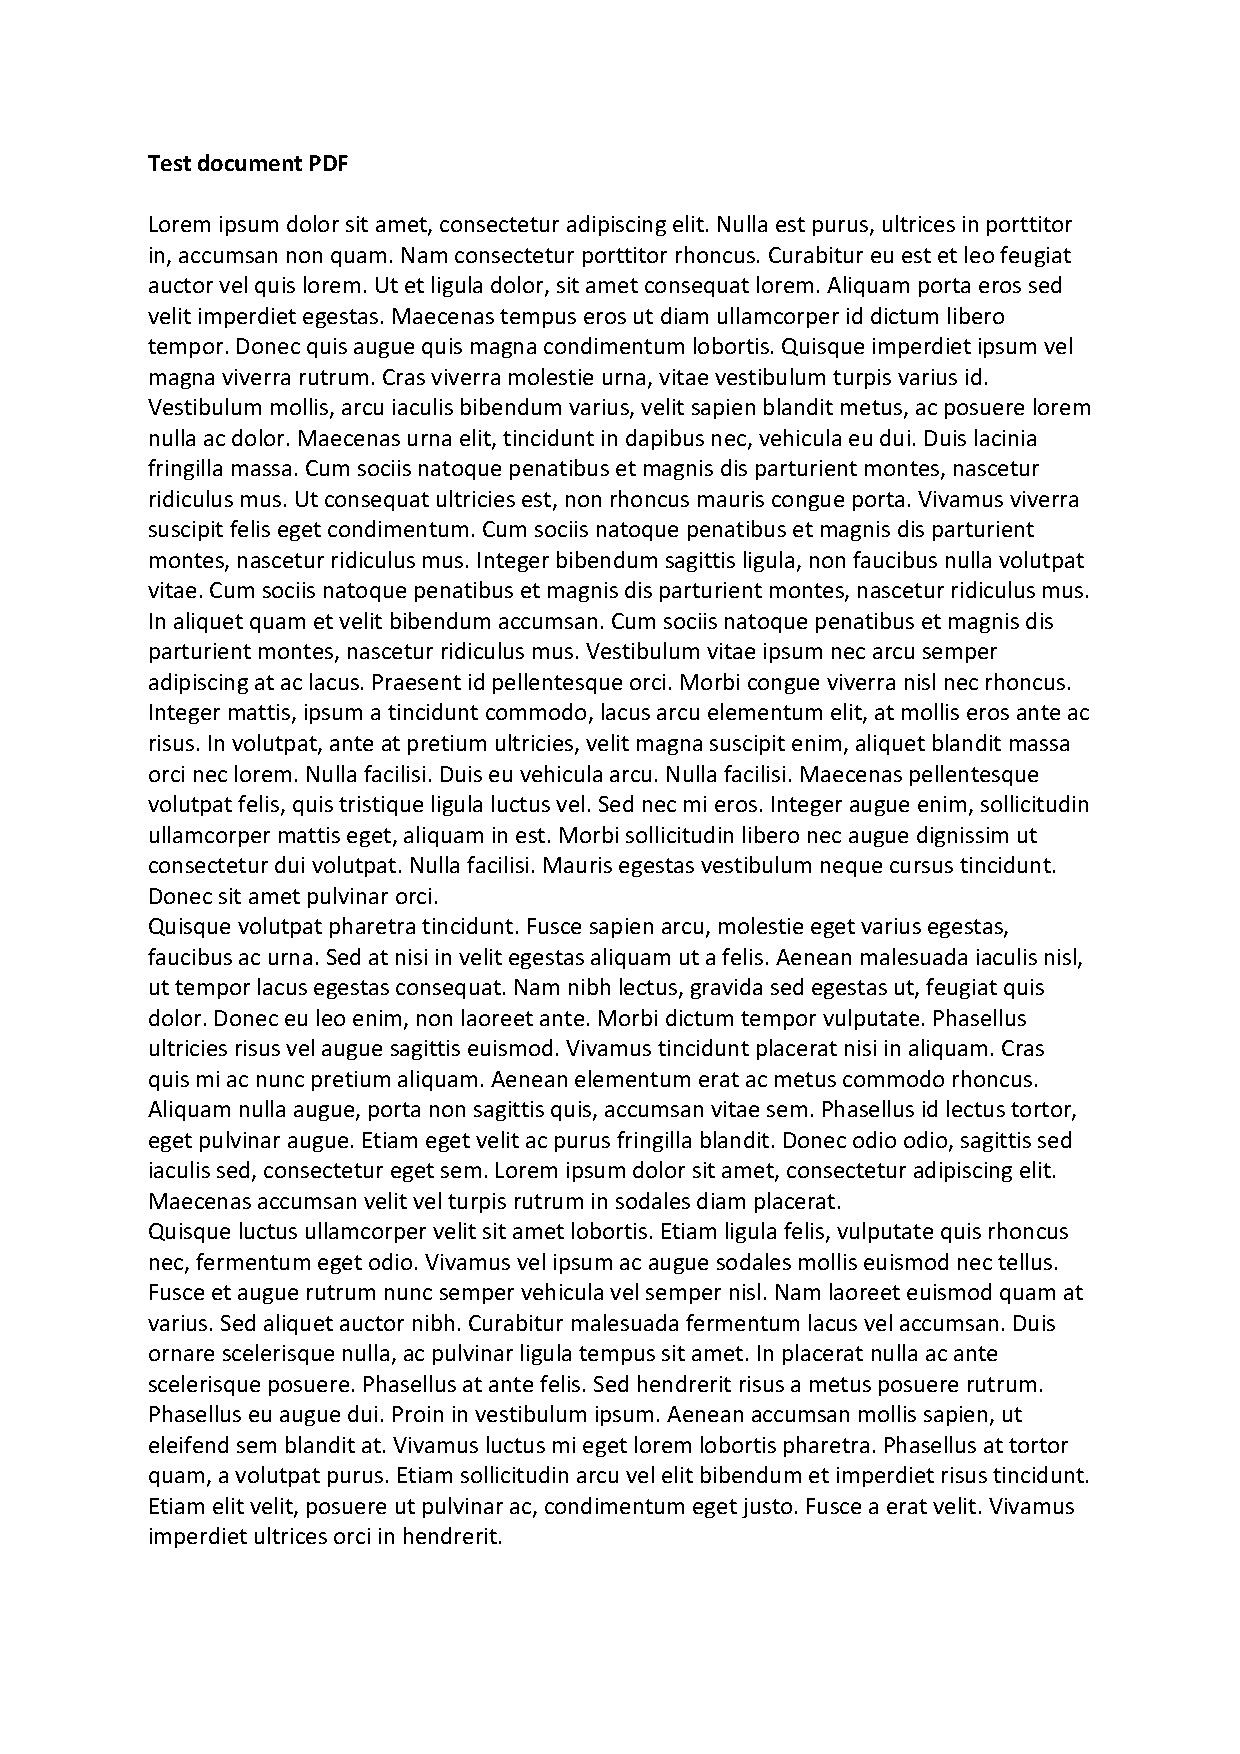
\includepdf[pages={1-last}, pagecommand={\pagestyle{fancyplain}}, height=1\textheight, clip, trim=15mm 10mm 15mm 5mm, offset=0 0]{contribution3-openml.pdf}



\chapter{OpenML Benchmarking Suites}
\label{chap:cont4}

Chapter \ref{chap:cont4} promotes the use of benchmarking suites (i.e., a carefully selected collection of easily accessible datasets).
The chapter also describes how researchers can create their own benchmarking suites on OpenML, and it presents a first such collection for classification datasets, namely the \textit{OpenML100} benchmarking suite.

\subsubsection*{Contributing article:}

\citationd

\subsubsection*{Author contributions:}

Explain what you and others did.


\newpage
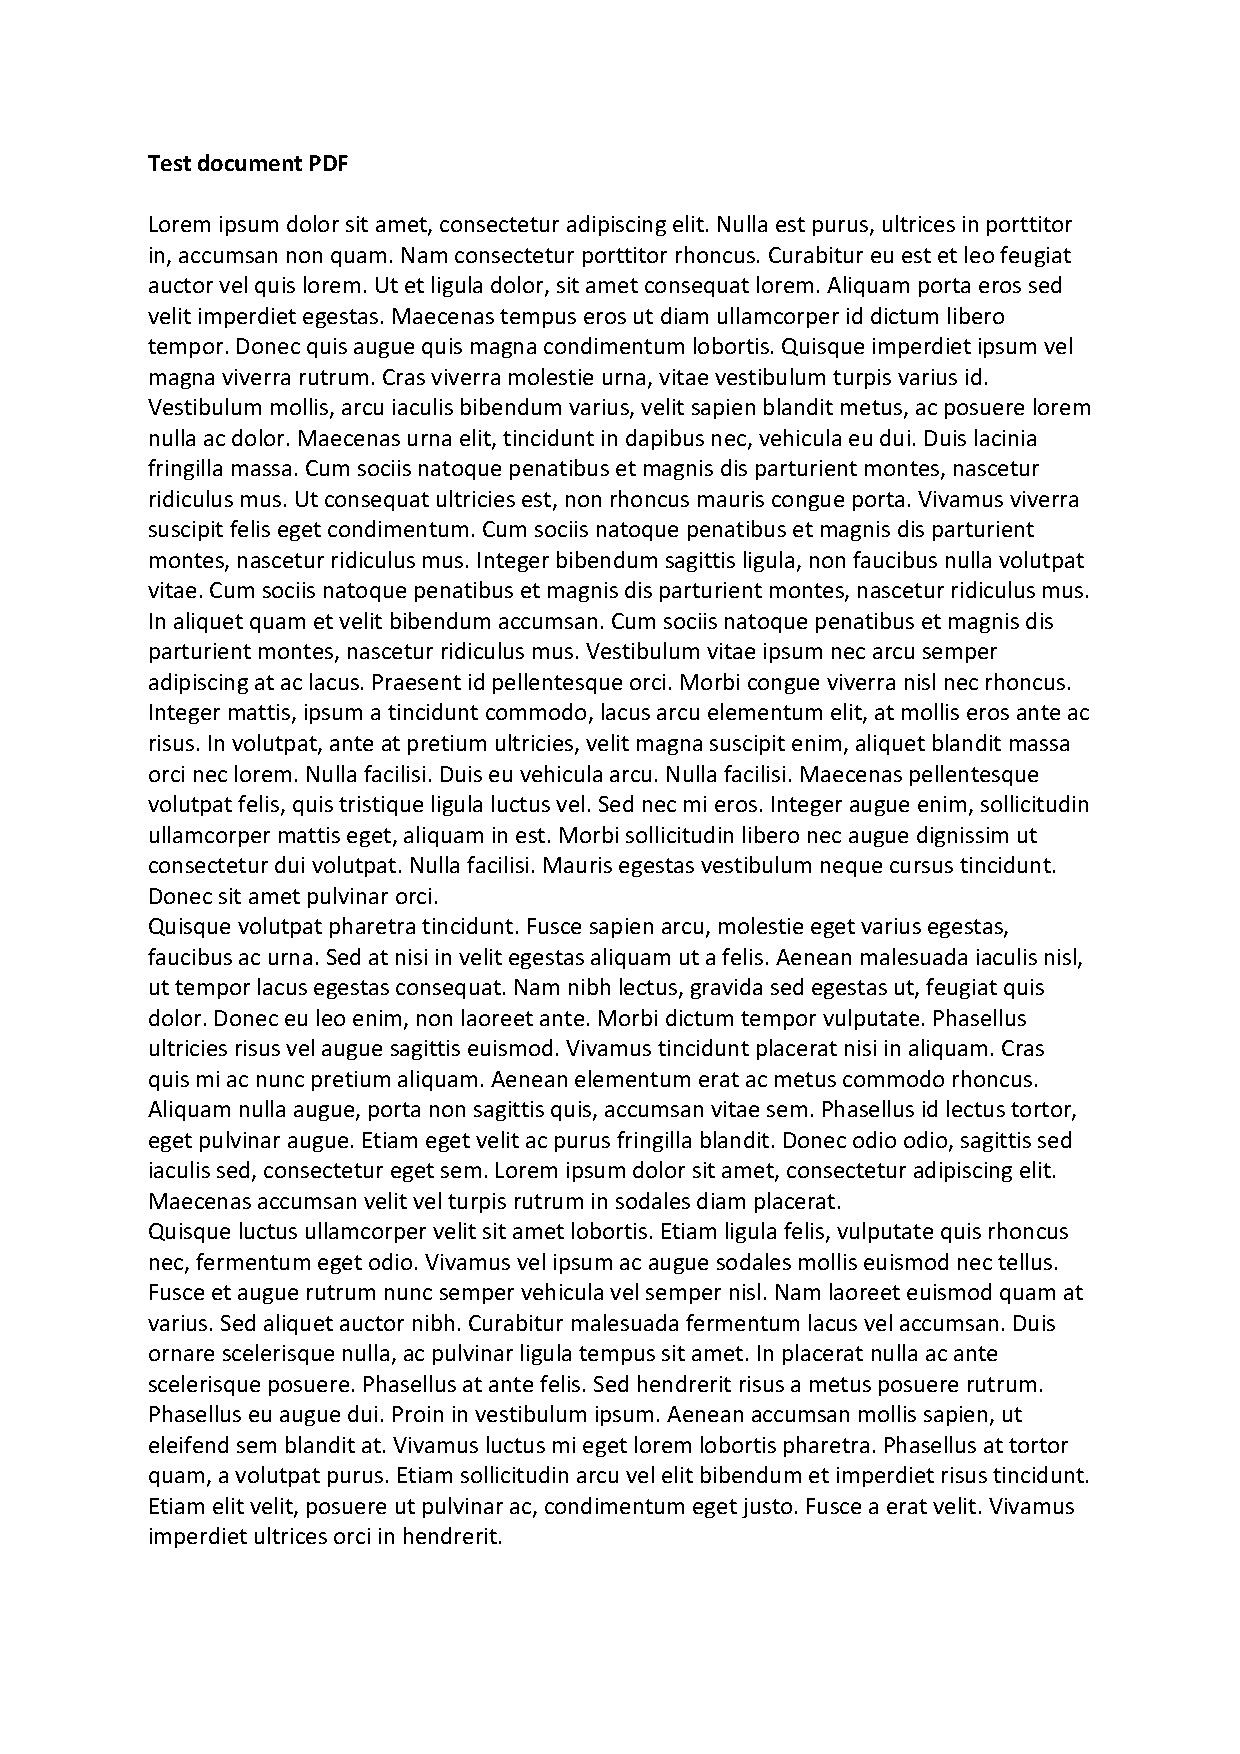
\includepdf[pages={1-last}, pagecommand={\pagestyle{fancyplain}}, height=1\textheight, clip, trim=30mm 20mm 30mm 10mm, offset=0 0]{contribution4-benchmark-suite.pdf}



\part{Evaluation and Interpretation of Machine Learning Models}
\label{part:iml}


\chapter{The Residual-Based Predictiveness Curve}
\label{chap:cont5}

The predictiveness curve \citep{Huang2007} is a visualization method to assess the performance of binary classifiers that predict probabilities.
Regarding the assessment of such probabilistic classifiers, two essential criteria must be considered, namely the discrimination performance and the calibration of the predicted probabilities.
The ROC curve is known to consider only the discrimination performance and not the calibration of the predicted probabilities.
Therefore, the use of the predictiveness curve is a reasonable alternative, since it also accounts for the calibration of the predicted probabilities \citep[cf.][]{Pepe2008b}.
Chapter \ref{chap:cont5} reviews the role of the predictiveness curve in the performance assessment and discusses several shortcomings of the curve.
Furthermore, the RBP curve is proposed as an extension that addresses several shortcomings of the original predictiveness curve.
This chapter also shows how the RBP curve can be used to derive several discrimination and calibration measures.

\subsubsection*{Contributing article:}

\citatione

\subsubsection*{Copyright information:}

%John Wiley & Sons, Inc. 2017.
The International Biometric Society, 2015.

\subsubsection*{Author contributions:}

Explain what you and others did.

\subsubsection*{Supplementary material available at:}

\begin{itemize}
\item \textsf{R} package: \url{https://cran.r-project.org/web/packages/RBPcurve}
\item Supplementary material: \newline \url{https://onlinelibrary.wiley.com/doi/abs/10.1111/biom.12455}
\end{itemize}



\newpage
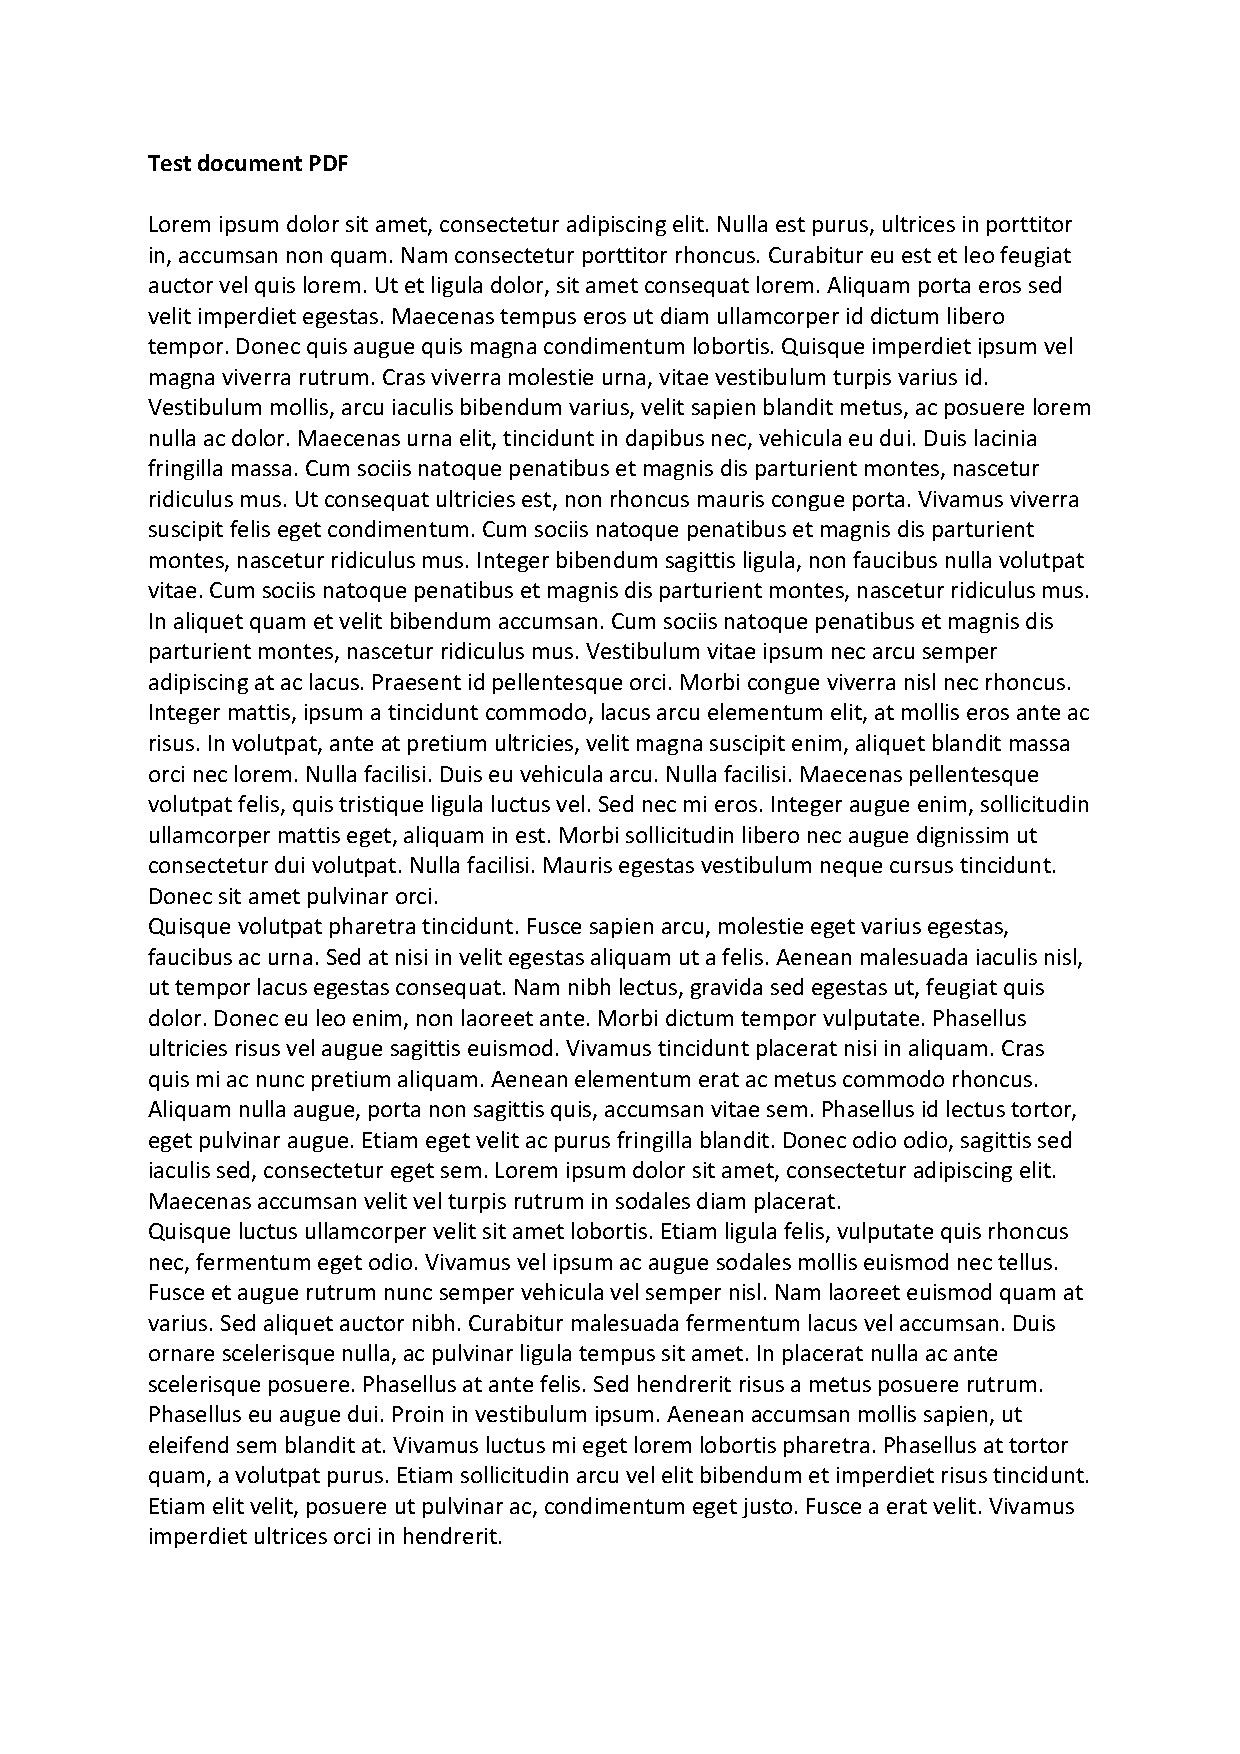
\includepdf[pages={1-last}, pagecommand={\pagestyle{fancyplain}}, width=1\textwidth, clip, trim=15mm 10mm 15mm 10mm, offset=0 0]{contribution5-rbp-curve.pdf}




\chapter{Visualizing the Feature Importance for Black Box Models}
\label{chap:cont6}

Chapter \ref{chap:cont6} first provides an overview of common model-agnostic interpretability methods in machine learning.
Furthermore, it introduces a local feature importance measure from which two novel visual tools are derived, namely the partial importance (PI) and individual conditional importance (ICI) plots.
The visual tools visualize how changes in a feature affect the model performance on average, as well as for individual observations.
Moreover, another feature importance measure called the Shapley feature importance (SFIMP) measure is introduced, which can be used to compare the feature importance across different models, since it fairly distributes the overall performance of a model among the features.

\subsubsection*{Contributing article:}

\citationf

\subsubsection*{Copyright information:}

\subsubsection*{Author contributions:}

Explain what you and others did.

\subsubsection*{Supplementary material available at:}

\textsf{R} package: \url{https://github.com/giuseppec/featureImportance}


\newpage
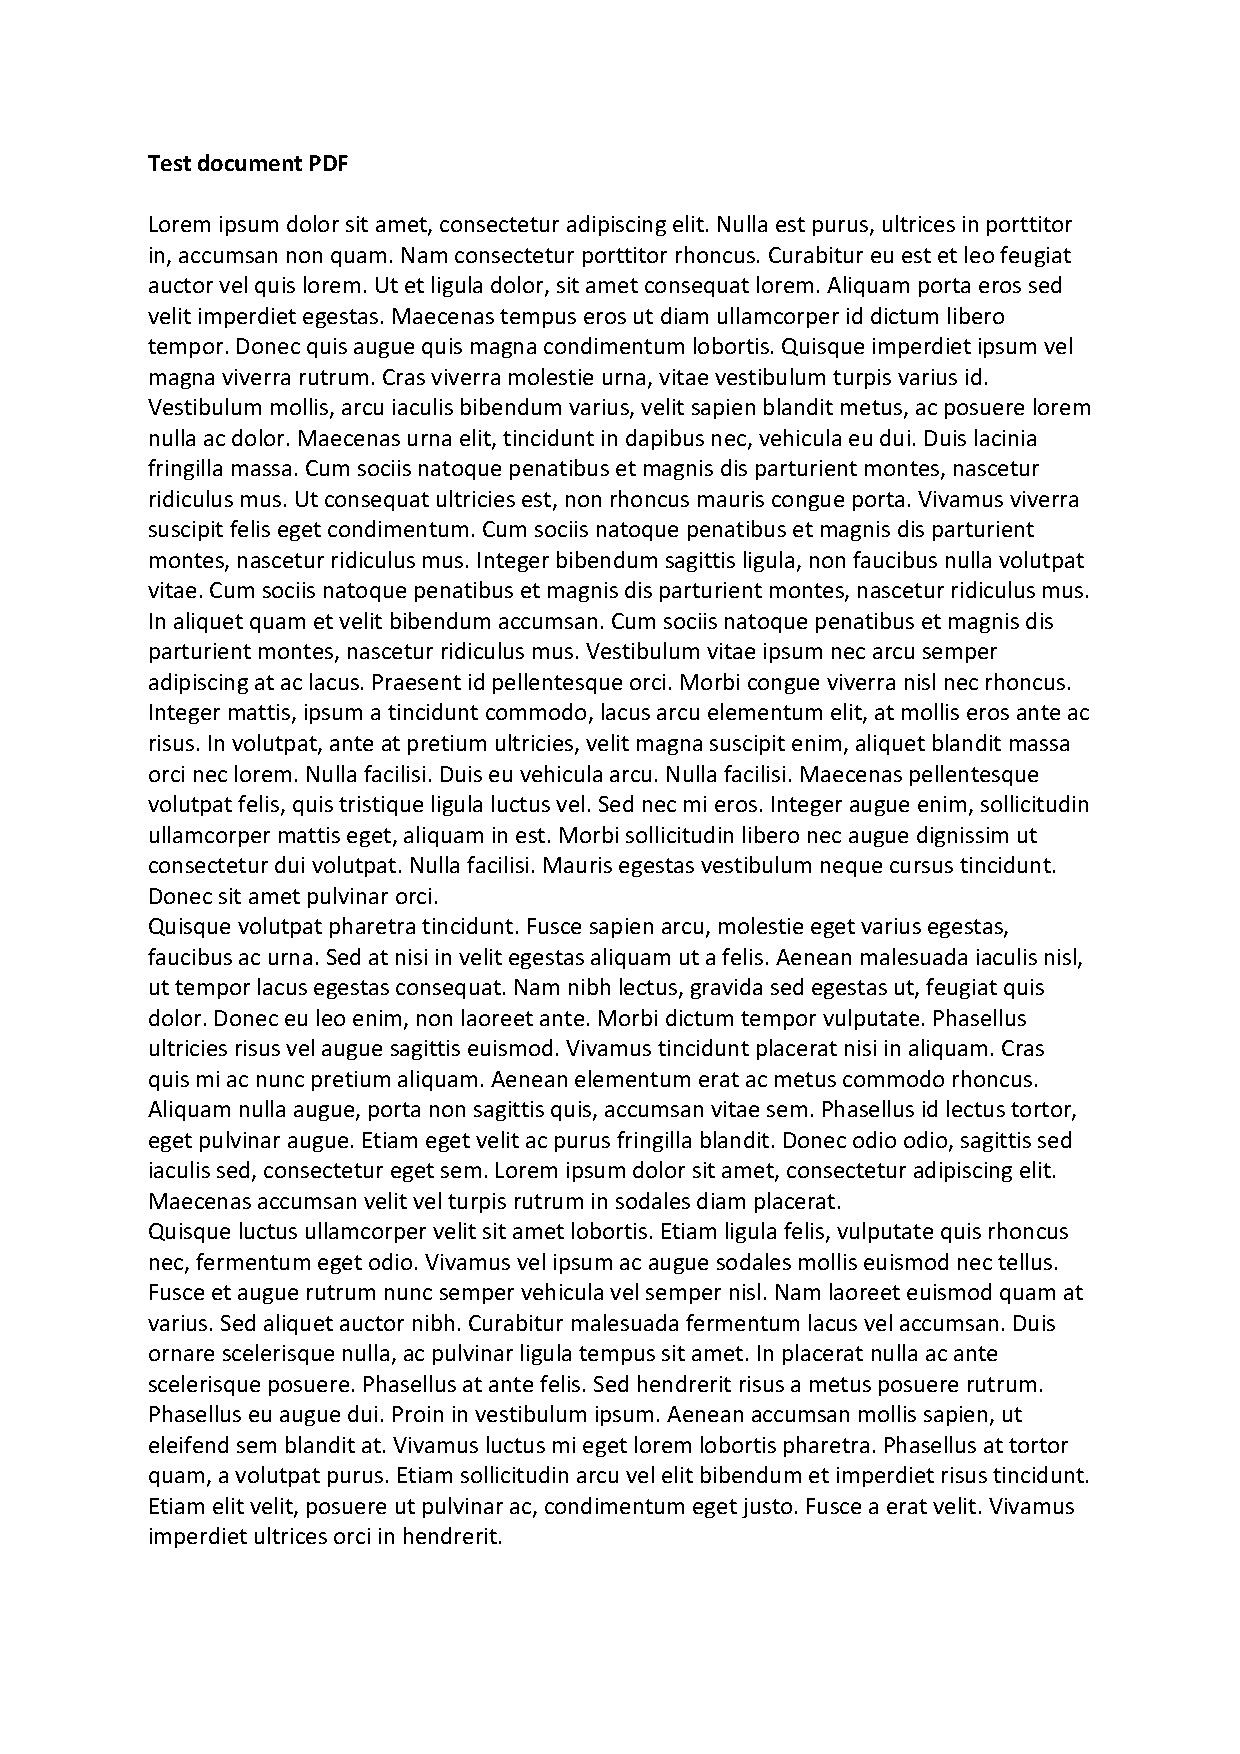
\includepdf[pages={1-last}, pagecommand={\pagestyle{fancyplain}}, height=1\textheight, clip, trim=46mm 60mm 38mm 30mm, offset=0 0]{contribution6-feature-importance.pdf}





\part{Conclusion}
\label{part:conclusion}

% Concluding Remarks
\chapter{Concluding Remarks and Future Work}

Final blabla

%%%%%%%%%%%%%%%%%%%%%%%%%%%%%%%%%
% References

% If you want to have your publications on a separate page
\renewcommand\bibname{\protect Contributing Publications}
\begin{thebibliography}{}
\bibitem[Probst et~al., 2017]{contribution2}
\citationb

\bibitem[Casalicchio et~al., 2017]{contribution3}
\citationc

\bibitem[Bischl et~al., 2017]{contribution4}
\citationd

\bibitem[Casalicchio et~al., 2016]{contribution5}
\citatione

\bibitem[Casalicchio et~al., 2018]{contribution6}
\citationf
\end{thebibliography}

\renewcommand\bibname{\protect Further References}
\bibliography{bib}



%%%%%%%%%%%%%%%%%%%%%%%%%%%%%%%%%
% Eidesstattliche Versicherung
\chapter*{Eidesstattliche Versicherung}
\thispagestyle{empty}
\vspace{-1cm}
(Siehe Promotionsordnung vom 12. Juli 2011, § 8 Abs. 2 Pkt. 5)

\vspace{2cm} Hiermit erkläre ich an Eides statt, dass die Dissertation von mir selbstständig, \\
ohne unerlaubte Beihilfe angefertigt ist.

\vspace{3cm}
\hfill\rule{6cm}{0.4pt}\\
\noindent München, den \deadline \hfill Giuseppe Casalicchio
\cleardoublepage

\end{document}
